\section{Checkpoint-on-Failure}\label{sect:cof}

% Teaser paragraph
Checkpoint-on-Failure (CoF)~\cite{Bland:2012tw} combines the familiarity of
checkpointing with the flexibility of \abft. As discussed in
Section~\ref{sect:related}, coordinated checkpointing is no longer considered a
scalable option for fault tolerance due to the increasing frequency and size of
the individual checkpoints. However, for some types of applications which can
take advantage of it, \cof can reduce the necessary number of checkpoints. In
the failure-free case, no checkpoints are made, and in all other cases, only the
optimal number of checkpoints are required.

% Define the "high-quality" implementation from the MPI Standard

The current MPI Standard (version 2.2~\cite{MPI22}) intentionally does not provide a
guideline for the behavior of the MPI library after a process failure. Section
2.8 states: ``\emph{MPI does not provide mechanisms for dealing with failures in
the communication system. [\ldots] Whenever possible, such failures will be
reflected as errors in the relevant communication call. Similarly, MPI itself
provides no mechanisms for handling processor failures.}'' Later, in the same
section: ``\emph{This document does not specify the state of a computation after
an erroneous MPI call has occurred. The desired behavior is that a relevant
error code be returned, and the effect of the error be localized to the greatest
possible extent.}'' Using these two sections from the standard, it is possible
to construct a minimal failure handling method using roll-forward recovery.

Section 8.3 (Error Handling) defines the behavior of a ``high quality''
implementation pertaining to error handling: ``\emph{A good quality
implementation will, to the greatest possible extent, circumscribe the impact of
an error, so that normal processing can continue after an error handler was
invoked.}'' By using a ``high quality'' MPI implementation as defined here, an
application will receive a notification from the MPI library through a custom
\mpifunc{MPI\_ERRHANDLER} when a failure occurs and before the library shuts
down operation. MPI makes no guarantee about the availability of the
communication library following a process failure, therefore standard
roll-forward recovery mechanisms are no longer possible. However, by using CoF
methods, an application still has an opportunity to save its state and exit
gracefully, then be restarted with the original number of processes and perform
recovery.

% Describe CoF in more detail

%\begin{algorithm*}
%\caption{The Checkpoint-on-Failure Protocol}
%\label{alg:on-demand-alg}\label{fig:cof-idea}
%\centering
%\begin{minipage}{.55\linewidth}
%	\begin{enumerate}
%		\item MPI returns an error on surviving processes 
%		\item Surviving processes checkpoint
%		\item Surviving processes exit
%		\item A new MPI application is started
%		\item Processes load from checkpoint (if any)
%		\item Processes enter \abft dataset recovery
%		\item Application resumes
%	\end{enumerate}
%\end{minipage}
%\hfill %\begin{minipage}{.39\linewidth}
%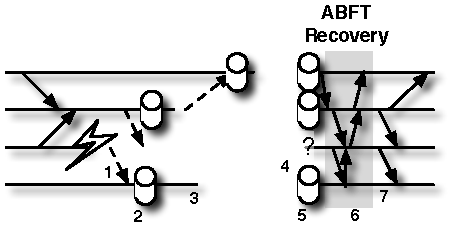
\includegraphics[width=\linewidth]{figures/cof-idea.pdf}
%\end{minipage}
%\end{algorithm*}

%Algorithm~\ref{alg:on-demand-alg}\footnote{Figure appeared
%in~\cite{Bland:2012tw}} presents the steps involved in the \cof method.
%Horizontal lines represent the execution of the MPI processes. 

The usage of the \cof model can be described as follows. When a failure
eliminates a process, other processes are notified and control is returned from
ongoing MPI calls. Surviving processes assume the MPI library is dysfunctional
as described in the MPI Standard and make no further calls to the MPI library
(in particular, they do not yet undergo \abft recovery). Instead, they
checkpoint their current state independently and abort. When all processes have
exited, the job is usually automatically terminated, and the user (or a managing
script, batch scheduler, runtime support system, etc.) can launch a new MPI
application, which reloads processes from checkpoint. In the new application,
the MPI library is functional and communication is once again possible; the
\abft recovery procedure is called to restore the data of the process(es) that
did not restart with a checkpoint (because they were the processes which
failed). When the global state has been repaired by the \abft procedure, the
application is ready to resume normal execution.

% Performance vs. periodic checkpointing

\cof has many advancements beyond traditional periodic checkpointing. First, it
is always optimized both in space and time. It takes checkpoints only after a
failure has occurred, meaning that there is no need to calculate an optimal
checkpoint interval~\cite{Daly:2006dy} or pause failure-free execution to write
state to disk. This can provide a measurable speedup in the application
performance, especially at scale because it reduces resource contention for the
I/O system. Also, because checkpoints are only written by processes which are
known to be alive, the checkpoint can be written to local stable storage rather
than requiring I/O be communicated between a remote, safe data store. The
overhead of \cof is also comparable to the standard overhead introduced by other
\abft techniques. The application might need to do extra computation, even in
the absence of failures, to maintain internal redundancy used to recover data
damaged by failures, however, this is necessary for all \abft techniques.

% MPI Requirements

\subsection{MPI Requirements for Checkpoint-on-Failure}\label{sec:interface}

\paragraph*{Regaining Control After Failures} In most MPI implementations,
\mpifunc{MPI\_ERRORS\_ABORT} is the default (and often, only functional) error
handler.  However, the MPI Standard also defines the error handler,
\mpifunc{MPI\_ERRORS\_RETURN} and provides mechanisms for custom error handlers
defined by the application. To support \cof, the MPI library should never
deadlock because of failures, but invoke the error handler, at least on
processes doing direct communications with the failed process. The error handler
takes care of cleaning up at the library level and returns control to the
application.

\paragraph*{Termination After Checkpoint} A process that detects a failure
ceases to use MPI. It checkpoints to storage, local or remote, and exits without
calling \mpifunc{MPI\_FINALIZE} (it may choose to call
\mpifunc{MPI\_COMM\_ABORT}, but this behavior is not required). Exiting without
calling \mpifunc{MPI\_FINALIZE} is an error from the MPI perspective, hence the
failure notification becomes fully propagated and MPI eventually calls the error
handler on all processes, which trigger their own checkpoint procedure and
termination.

\subsection{\ompi Implementation\label{sec:mpi}}

\ompi is an MPI 2.2 implementation architected such that it contains two main
levels, the runtime (ORTE) and the MPI library (OMPI). As with most MPI library
implementations, the default behavior of \ompi is to abort after a process
failure. This policy was implemented in the runtime system, preventing any kind
of decision from the MPI layer or the user level. The major change required by
the \cof protocol was to make the runtime system resilient, leaving the policy
for failure handling to the MPI library, and ultimately the user application.

\paragraph*{Resilient Runtime} The ORTE runtime layer provides an out-of-band
(OOB) communication mechanism that relays messages based on a routing policy.
Node failures not only impact the MPI communications, but also disrupt routing
at the OOB level. The default routing policy in ORTE has been amended to allow
for self-healing behaviors; this effort is not entirely necessary, but it avoids
the significant downtime imposed by a complete redeployment of the parallel job
with resubmission into execution queues. The underlying OOB topology is
automatically updated to route around failed processes. In some routing
topologies, such as a star, this is a trivial operation and only requires
excluding the failed process from the routing tables. For more elaborate
topologies, such as trees, the healing operation involves computing
the closest neighbors in the direction of the failed process and reconnecting
the topology through them. The repaired topology is not rebalanced, which could
result in improved performance but would disrupt expected communication
patterns, however it does retain complete functionality to allow the MPI
implementation to maintain internal communication and facilitate failure
notification. Although in-flight messages that were currently ``hopping''
through the failed processes are lost, other in-flight messages are safely
routed by the repaired topology. Thanks to self-healing topologies, the runtime
remains responsive, even when MPI processes leave.

\paragraph*{Failure Notification} The runtime has been further augmented with a
failure detection service. To track the status of the failures, an incarnation
number has been included in the process names. Following a failure, the name of
the failed process (including the incarnation number) is broadcasted over the
OOB topology. By including this incarnation number, we can identify transient
process failures, prevent duplicate detections, and track message status. ORTE
processes monitor the health of their neighbors in the OOB routing topology.
Process failure detection relies on a resilient broadcast operation that
overlays on the OOB topology. However, the underlying OOB routing algorithm has
a significant influence on failure detection and propagation time, as the
experiments will show. On each node, the ORTE runtime layer forwards failure
notifications to the MPI layer, which has been modified to invoke the
appropriate MPI error handler.

